\chapter{Report di Qualità del Codice}
La qualità del codice rappresenta un elemento fondamentale nello sviluppo software.
Un codice di alta qualità facilita la comprensione e la manutenzione da parte degli sviluppatori, riduce il numero di bug e vulnerabilità, aumentando la stabilità dell'applicazione.\par
Inoltre, un codice ben strutturato e pulito è essenziale per garantire la scalabilità del progetto. Permette di aggiungere nuove funzionalità senza compromettere le performance o l'affidabilità del sistema.

\section{SonarQube}
Per monitorare e migliorare la qualità del codice, è stato impiegato SonarQube. Questo permette di identificare potenziali bug, vulnerabilità e problemi tecnici, fornendo suggerimenti per ottimizzare il codice.
\begin{itemize}
    \item \textbf{Duplicazioni}: Le duplicazioni di codice possono portare a una maggiore complessità e difficoltà nella manutenzione. SonarQube rileva segmenti di codice duplicati e suggerisce di refattorizzarli per migliorare l'efficienza e ridurre il rischio di inconsistenze.

    \item \textbf{Bugs}: Rappresentano errori nel codice che possono causare comportamenti imprevisti o malfunzionamenti dell'applicazione.

    \item \textbf{Vulnerabilità}: Questi indici segnalano potenziali rischi di sicurezza presenti nel codice.
    
    \item \textbf{Code Smells}: Indicano aree del codice che, pur non essendo errori diretti, possono ridurre la leggibilità, la manutenibilità o la performance dell'applicazione.
\end{itemize}
\pagebreak
\subsection*{Duplicazioni}
Nel nostro progetto, il grafico delle duplicazioni di codice si è mantenuto costante nel tempo, nonostante l'incremento delle linee di codice complessive. Questo andamento positivo indica che, anche con la crescita del codice, siamo riusciti a gestire efficacemente la duplicazione, mantenendo un livello di duplicazione sotto controllo.\meskip
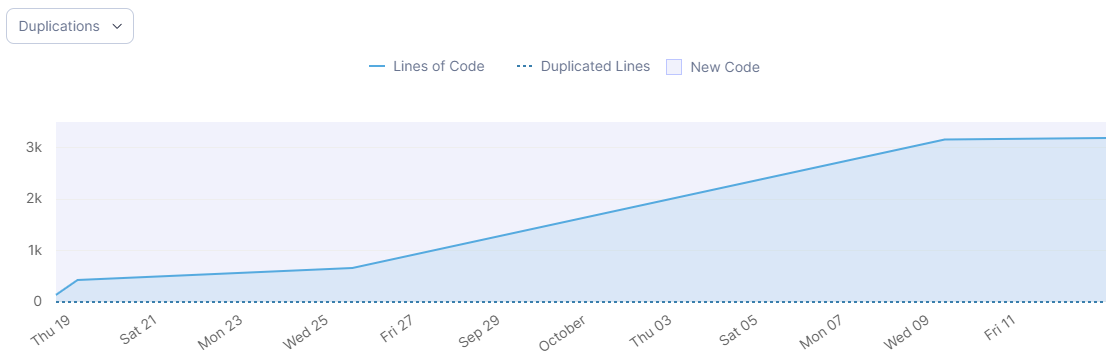
\includegraphics[width=\textwidth]{assets/sonarqube/duplication.png}

\subsection*{Errori}
Il grafico degli errori del nostro progetto presenta un andamento particolarmente positivo: inizia con un numero elevato di \textit{code smells} e mostra una costante diminuzione fino a raggiungere lo zero.\par
La diminuzione degli errori nel codice ha incrementato la stabilità dell'applicazione e riducendo i malfunzionamenti. Inoltre, ha facilitato la manutenzione e l'evoluzione del software, permettendo di aggiungere nuove funzionalità con maggiore sicurezza e minor rischio di introdurre nuovi bug.\meskip
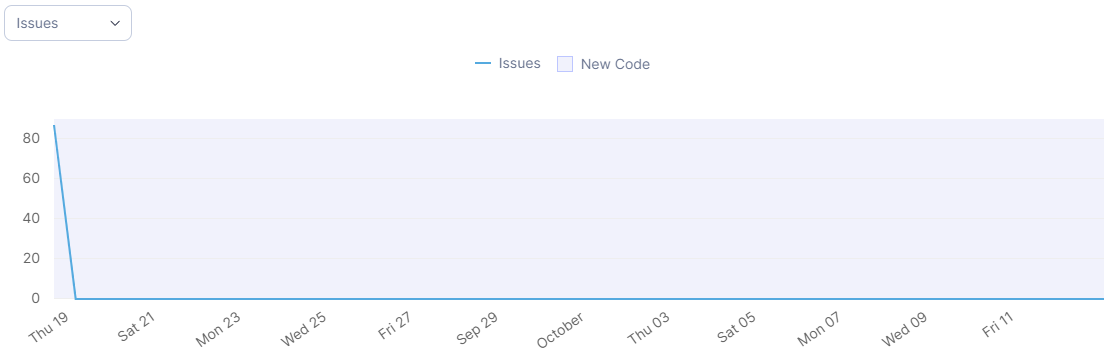
\includegraphics[width=\textwidth]{assets/sonarqube/issues.png}